\documentclass{mcmthesis}
\mcmsetup{CTeX = false,   % 使用 CTeX 套装时,设置为 true
        tcn = 0000, problem = B,
        sheet = false, titleinsheet = true, keywordsinsheet = true,
        titlepage = true, abstract = true}
\usepackage{newtxtext}%\usepackage{palatino}
\usepackage{lipsum}
\title{Mathematical Modeling of Wildfire Evacuation in Maui, Hawaii}

\date{\today}
\begin{document}
\begin{abstract}
In this paper, we present a mathematical model for wildfire evacuation in Maui, Hawaii, based on cellular automata principles. Our model consists of two sub-models: a wildfire propagation model and an evacuation model. The wildfire propagation model simulates the spread of fire on a grid of cells, where each cell represents a unit of land with certain attributes, such as vegetation type, moisture level, and elevation. The fire spread is influenced by factors such as wind speed, wind direction, temperature, and humidity. The evacuation model simulates the movement of people on a road network, where each node represents an intersection or an evacuation point, and each edge represents a road segment. The evacuation model considers the population distribution, the evacuation routes, the evacuation points, and the traffic flow in different regions. The model also incorporates the effects of factors like drought, hurricanes, and vegetation changes on the wildfire risk and the evacuation process.

\begin{keywords}
keyword1; keyword2
\end{keywords}
\end{abstract}
\maketitle

\tableofcontents
\newpage
%%
%% Generate the Memorandum, if it's needed.
%% \memoto{\LaTeX{}studio}
%% \memofrom{Liam Huang}
%% \memosubject{Happy \TeX{}ing!}
%% \memodate{\today}
%% \logo{\LARGE I'm pretending to be a LOGO!}
%% \begin{memo}[Memorandum]
%%   \lipsum[1-3]
%% \end{memo}
%%
\section{Introduction}
\subsection{The condition of Maui}
Maui, Hawaii, located in the central Pacific, is renowned for its stunning natural landscapes and diverse vegetation, making it a popular tourist destination. However, the island faces increased wildfire risks due to factors such as drought, hurricanes, vegetation changes, and a scarcity of firefighters. According to the Hawaii Wildfire Management Organization, wildfires have burned over 25\% of Hawaii's total land area since 2000, and Maui has experienced some of the largest and most destructive fires in the state's history. To ensure the safety of residents and tourists, there is a need to develop a wildfire evacuation model for planning evacuation strategies during wildfire events.
\subsection{The models of Cellular Automata}
Cellular automata (CA) are discrete mathematical models that consist of a grid of cells, each of which can have a finite number of states, and a set of rules that determine the state transition of each cell based on its neighborhood. CA have been widely used to model complex phenomena such as fluid dynamics, traffic flow, urban growth, and biological systems . In particular, CA have been applied to model wildfire propagation and evacuation, as they can capture the spatial and temporal dynamics of fire spread and human behavior. However, most of the existing CA models for wildfire evacuation are either too simplistic or too specific, and do not consider the effects of various factors that affect wildfire risk and evacuation efficiency in Maui.
\subsection{Our work}
In this paper, we aim to address this gap by presenting a comprehensive and realistic CA model for wildfire evacuation in Maui, Hawaii. Our model consists of four sub-models: a wildfire propagation sub-model, an evacuation sub-model, a firefighter deployment sub-model, and a risk assessment sub-model. We use the model to answer the following questions:
\lipsum[3]
\begin{itemize}
\item How fast and how far will the wildfire spread under different conditions?
\item What is the best evacuation strategy to minimize the risk of casualties among affected populations?
\item How should the firefighter resources be allocated to effectively contain the spread of wildfires?
\item How much time is required for residents and tourists in different areas to safely evacuate?
\item How can the impact of factors such as drought, hurricanes, and vegetation changes on wildfire risk be assessed?
\item How can an early warning system be established to notify residents and tourists in advance?
\end{itemize}

\section{Analysis of the Problem}
\begin{figure}[h]
\small
\centering
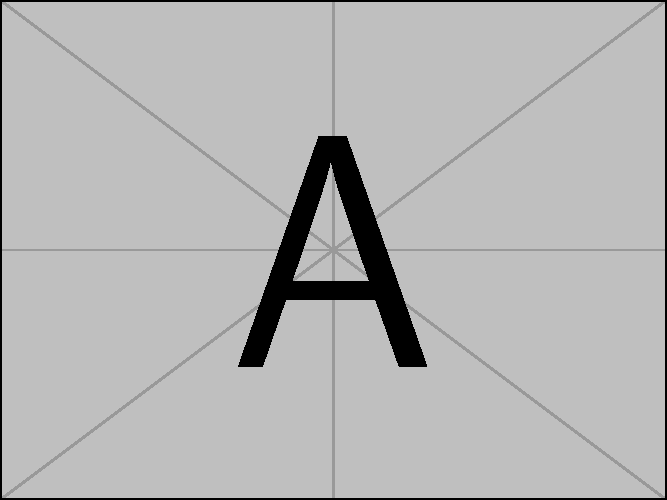
\includegraphics[width=8cm]{example-image-a}
\caption{The name of figure} \label{fig:aa}
\end{figure}

\lipsum[8] \eqref{aa}
\begin{equation}
a^2 \label{aa}
\end{equation}

\[
  \begin{pmatrix}{*{20}c}
  {a_{11} } & {a_{12} } & {a_{13} }  \\
  {a_{21} } & {a_{22} } & {a_{23} }  \\
  {a_{31} } & {a_{32} } & {a_{33} }  \\
  \end{pmatrix}
  = \frac{{Opposite}}{{Hypotenuse}}\cos ^{ - 1} \theta \arcsin \theta
\]
\lipsum[9]

\[
  p_{j}=\begin{cases} 0,&\text{if $j$ is odd}\\
  r!\,(-1)^{j/2},&\text{if $j$ is even}
  \end{cases}
\]

\lipsum[10]

\[
  \arcsin \theta  =
  \mathop{{\int\!\!\!\!\!\int\!\!\!\!\!\int}\mkern-31.2mu
  \bigodot}\limits_\varphi
  {\mathop {\lim }\limits_{x \to \infty } \frac{{n!}}{{r!\left( {n - r}
  \right)!}}} \eqno (1)
\]

\section{Calculating and Simplifying the Model  }
\lipsum[11]

\section{The Model Results}
\lipsum[6]

\section{Validating the Model}
\lipsum[9]

\section{Conclusions}
\lipsum[6]

\section{A Summary}
\lipsum[6]

\section{Evaluate of the Mode}

\section{Strengths and weaknesses}
\lipsum[12]

\subsection{Strengths}
\begin{itemize}
\item \textbf{Applies widely}\\
This  system can be used for many types of airplanes, and it also
solves the interference during  the procedure of the boarding
airplane,as described above we can get to the  optimization
boarding time.We also know that all the service is automate.
\item \textbf{Improve the quality of the airport service}\\
Balancing the cost of the cost and the benefit, it will bring in
more convenient  for airport and passengers.It also saves many
human resources for the airline. \item \textbf{}
\end{itemize}

\begin{thebibliography}{99}
\bibitem{1} D.~E. KNUTH   The \TeX{}book  the American
Mathematical Society and Addison-Wesley
Publishing Company , 1984-1986.
\bibitem{2}Lamport, Leslie,  \LaTeX{}: `` A Document Preparation System '',
Addison-Wesley Publishing Company, 1986.
\bibitem{3}\url{https://www.latexstudio.net/}
\end{thebibliography}

\begin{appendices}

\section{First appendix}

In addition, your report must include a letter to the Chief Financial Officer (CFO) of the Goodgrant Foundation, Mr. Alpha Chiang, that describes the optimal investment strategy, your modeling approach and major results, and a brief discussion of your proposed concept of a return-on-investment (ROI). This letter should be no more than two pages in length.

\begin{letter}{Dear, Mr. Alpha Chiang}

\lipsum[1-2]

\vspace{\parskip}

Sincerely yours,

Your friends

\end{letter}
Here are simulation programmes we used in our model as follow.\\

\textbf{\textcolor[rgb]{0.98,0.00,0.00}{Input matlab source:}}
\lstinputlisting[language=Matlab]{./code/mcmthesis-matlab1.m}

\section{Second appendix}

some more text \textcolor[rgb]{0.98,0.00,0.00}{\textbf{Input C++ source:}}
\lstinputlisting[language=C++]{./code/mcmthesis-sudoku.cpp}

\end{appendices}
\end{document}
%% 
%% This work consists of these files mcmthesis.dtx,
%%                                   figures/ and
%%                                   code/,
%% and the derived files             mcmthesis.cls,
%%                                   mcmthesis-demo.tex,
%%                                   README,
%%                                   LICENSE,
%%                                   mcmthesis.pdf and
%%                                   mcmthesis-demo.pdf.
%%
%% End of file `mcmthesis-demo.tex'.
